\section{Volatility forecasting}
\label{sec:forecasting}

\subsection{Forecasting dataset and temporal split}

The forecasting experiment evaluates whether RMT and network features contain incremental information for realized volatility. The experiment is deliberately conservative. It uses PETR4, VALE3 and BBDC4 as target assets and compares network-augmented machine-learning models with strong econometric baselines. The data are split temporally: training covers 2006--2017, validation covers 2018--2020 and testing covers 2021--2025. This temporal split is designed to reduce look-ahead bias and to evaluate model selection on observations later than those used for training. Because some network and RMT features are based on static or slowly changing structures, the forecasting experiment is interpreted as an incremental-information test rather than as a fully real-time trading design.

\subsection{GARCH persistence and econometric benchmarks}

The GARCH(1,1) estimates with Student-$t$ innovations indicate high volatility persistence. Table~\ref{tab:garch_params} reports $\omega$, $\alpha$, $\beta$ and $\alpha+\beta$. The persistence values are 0.9911 for PETR4, 0.9946 for VALE3 and 0.9828 for BBDC4. All three estimates satisfy $\alpha+\beta<1$, but the values are close to unity, indicating highly persistent conditional variance dynamics. These high values help explain why classical volatility benchmarks are difficult to outperform and are consistent with the slow decay of absolute-return autocorrelations documented in Section~\ref{sec:stylized_correlation}.

\begin{center}
\captionof{table}{GARCH(1,1) persistence estimates for the forecasting assets.}
\label{tab:garch_params}
\begin{tabular}{lrrrr}
\toprule
Asset & $\omega$ & $\alpha$ & $\beta$ & $\alpha+\beta$ \\
\midrule
BBDC4 & 0.0729 & 0.0520 & 0.9308 & 0.9828 \\
PETR4 & 0.0780 & 0.0758 & 0.9153 & 0.9911 \\
VALE3 & 0.0417 & 0.0512 & 0.9434 & 0.9946 \\
\bottomrule
\end{tabular}
\end{center}

\subsection{Machine-learning feature sets}

The machine-learning models use three nested feature sets in an ablation design. Set~A contains classical volatility features. Set~B adds market and RMT variables. Set~C adds MST and PMFG network variables. This nesting allows the experiment to assess whether network topology adds incremental information beyond classical lagged-volatility persistence and broad market/RMT features.

\subsection{Out-of-sample model comparison}

Figure~\ref{fig:forecast_comparison} summarizes out-of-sample QLIKE loss. Lower QLIKE is better. For machine-learning models, the reported feature set is selected using the validation period and then evaluated on the test period.

\begin{center}
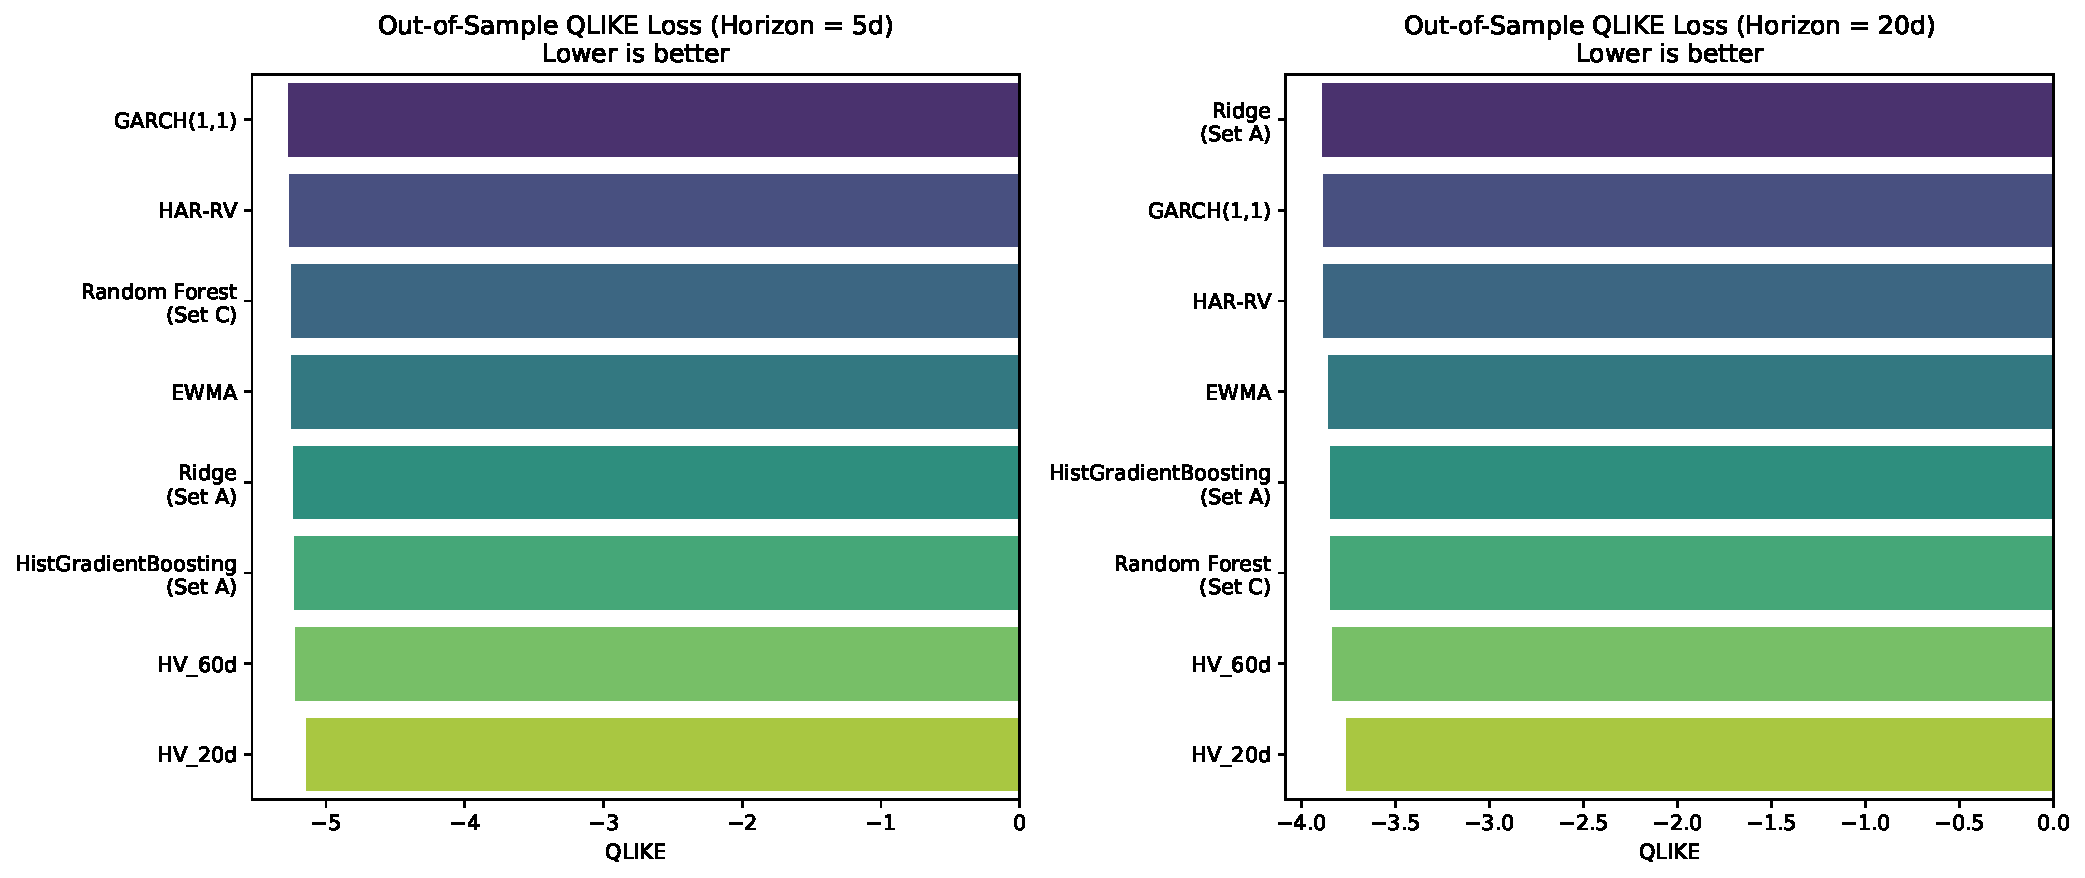
\includegraphics[
  width=\linewidth,
  height=0.58\textheight,
  keepaspectratio
]{images/figure_16_volatility_forecast_model_comparison.pdf}
\captionof{figure}{Volatility forecasting comparison for econometric and machine-learning models. Machine-learning labels show the best feature set selected for each model and horizon.}
\label{fig:forecast_comparison}
\end{center}

At the 5-day horizon, GARCH(1,1), HAR-RV and Random Forest are highly competitive. GARCH has average test QLIKE close to -5.27, HAR-RV is close to -5.26 and Random Forest with Set~C is close to -5.25. The differences are small; therefore, the appropriate interpretation is not that machine learning dominates, but that the network-augmented Random Forest reaches performance comparable to strong classical benchmarks.

At the 20-day horizon, Ridge models with Set~A or Set~B obtain slightly lower average QLIKE than GARCH in this experiment. Ridge Set~A and Set~B are close to -3.89, while GARCH is close to -3.88. No formal equal-predictive-ability test is reported, so these differences should be interpreted descriptively. Random Forest Set~C remains competitive but does not dominate. This result suggests that longer-horizon volatility may be easier to forecast with stable linear shrinkage features, while nonlinear models require careful regularization and validation.

\begin{center}
\captionof{table}{Aggregated test-set forecasting comparison (2021--2025). Values are averaged across PETR4, VALE3 and BBDC4.}
\label{tab:forecast_comparison}
\resizebox{\linewidth}{!}{%
\begin{tabular}{llrrrrr}
\toprule
Horizon & Model & Feature set & MAE & RMSE & QLIKE & $R^2_{\mathrm{oos}}$ \\
\midrule
5 & GARCH(1,1) & Classical & 0.0156 & 0.0213 & $-5.2700$ & 0.1600 \\
5 & HAR-RV & Classical & 0.0148 & 0.0198 & $-5.2600$ & 0.2200 \\
5 & Random Forest & Set C (+Network) & 0.0151 & 0.0204 & $-5.2500$ & 0.2000 \\
5 & EWMA & Classical & 0.0153 & 0.0207 & $-5.2500$ & 0.1900 \\
20 & Ridge & Set A (Classical) & 0.0241 & 0.0328 & $-3.8900$ & 0.3900 \\
20 & Ridge & Set B (+Market/RMT) & 0.0242 & 0.0329 & $-3.8900$ & 0.3900 \\
20 & GARCH(1,1) & Classical & 0.0278 & 0.0381 & $-3.8800$ & 0.2300 \\
20 & HAR-RV & Classical & 0.0260 & 0.0356 & $-3.8800$ & 0.2800 \\
20 & Random Forest & Set C (+Network) & 0.0287 & 0.0393 & $-3.8500$ & 0.1700 \\
\bottomrule
\end{tabular}}
\end{center}

\subsection{Realized vs predicted volatility diagnostics}

Aggregate metrics can hide important time-series behaviour. Figure~\ref{fig:realized_vs_predicted} compares realized 20-day volatility with GARCH and Random Forest forecasts for PETR4, VALE3 and BBDC4. This diagnostic is included in the main text because it illustrates how forecasts track changing volatility regimes.

\begin{center}
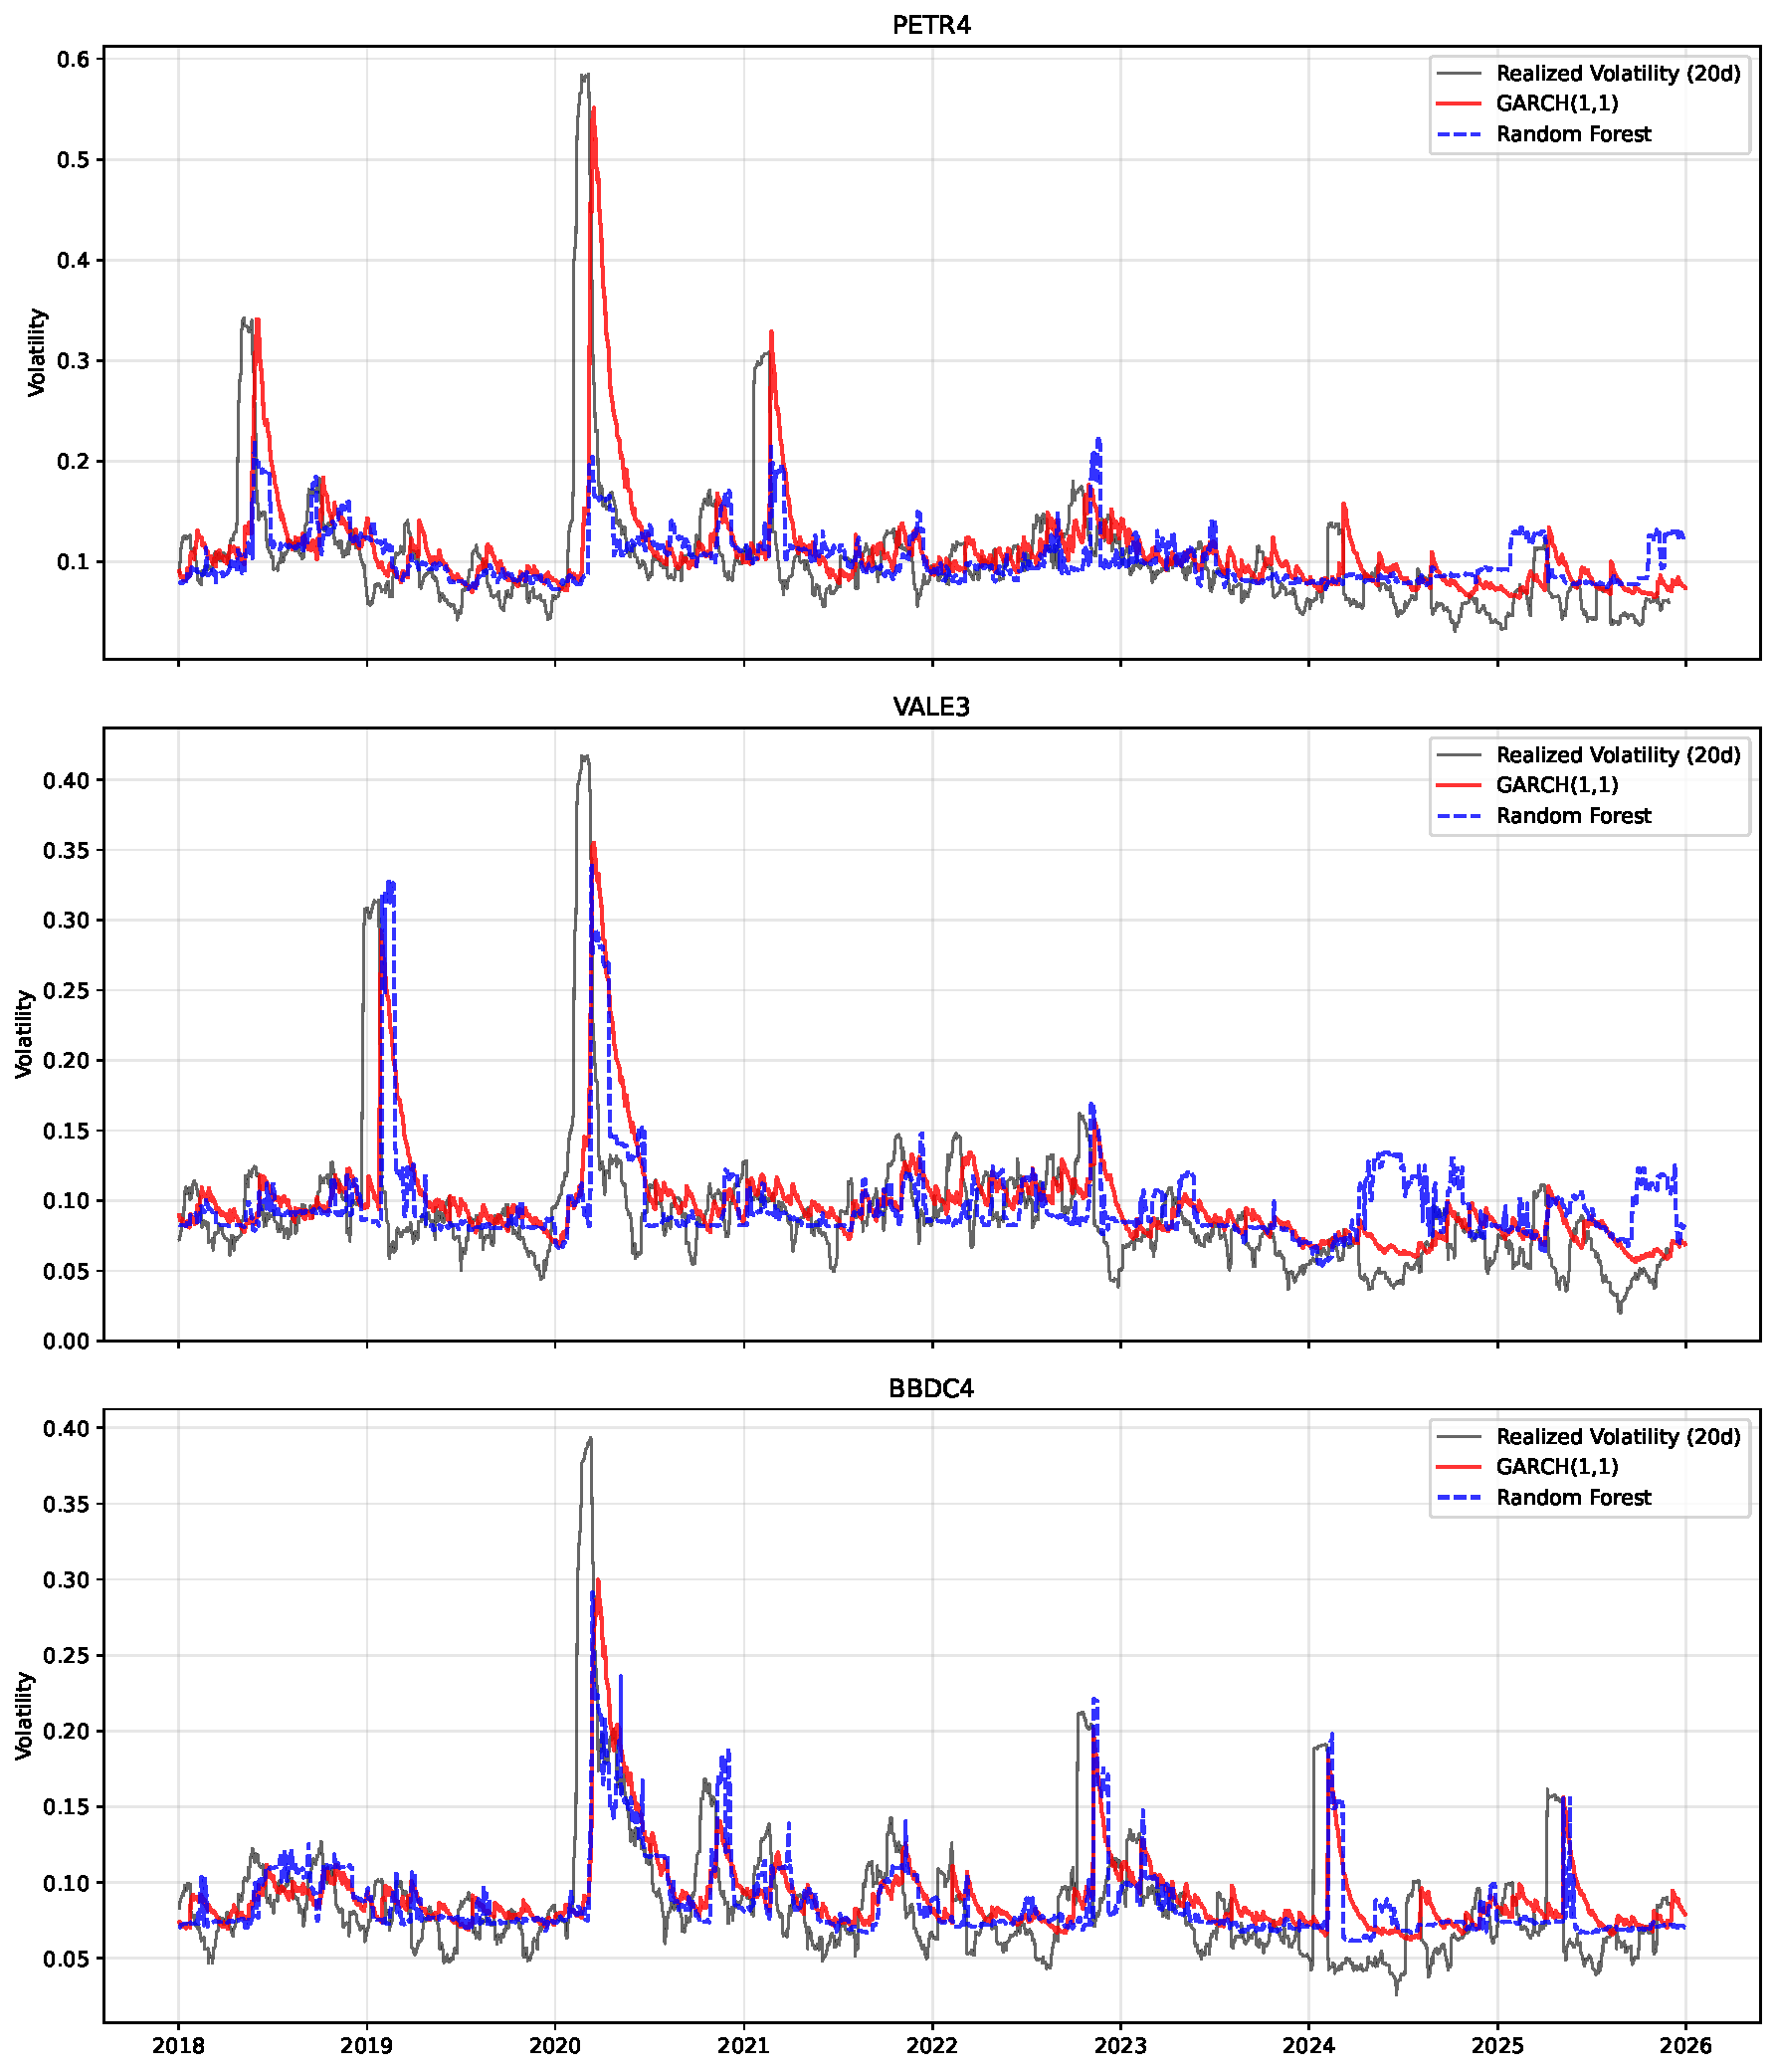
\includegraphics[
  width=0.95\linewidth,
  height=0.58\textheight,
  keepaspectratio
]{images/figure_17_realized_vs_predicted_volatility.pdf}
\captionof{figure}{Realized versus predicted 20-day volatility for selected models and assets. The plot illustrates regime tracking and forecast smoothness.}
\label{fig:realized_vs_predicted}
\end{center}

The diagnostic plots suggest that broad volatility regimes are tracked reasonably well, but extreme spikes remain difficult to forecast. GARCH forecasts respond through the persistence of conditional variance, while Random Forest forecasts can appear smoother or more step-like because tree-based predictions are piecewise constant over feature regions. This behaviour is consistent with the aggregate results: nonlinear models can be competitive, but lagged volatility and volatility persistence remain the main sources of predictive information.

\subsection{Feature importance and network signal}

Random Forest feature importance provides a model-specific diagnostic of which predictors contribute most to the fitted model. Figure~\ref{fig:feature_importance} shows that classical volatility features dominate the model. Rolling absolute returns, lagged realized volatility, rolling volatility and EWMA variables carry most of the importance.

\begin{center}
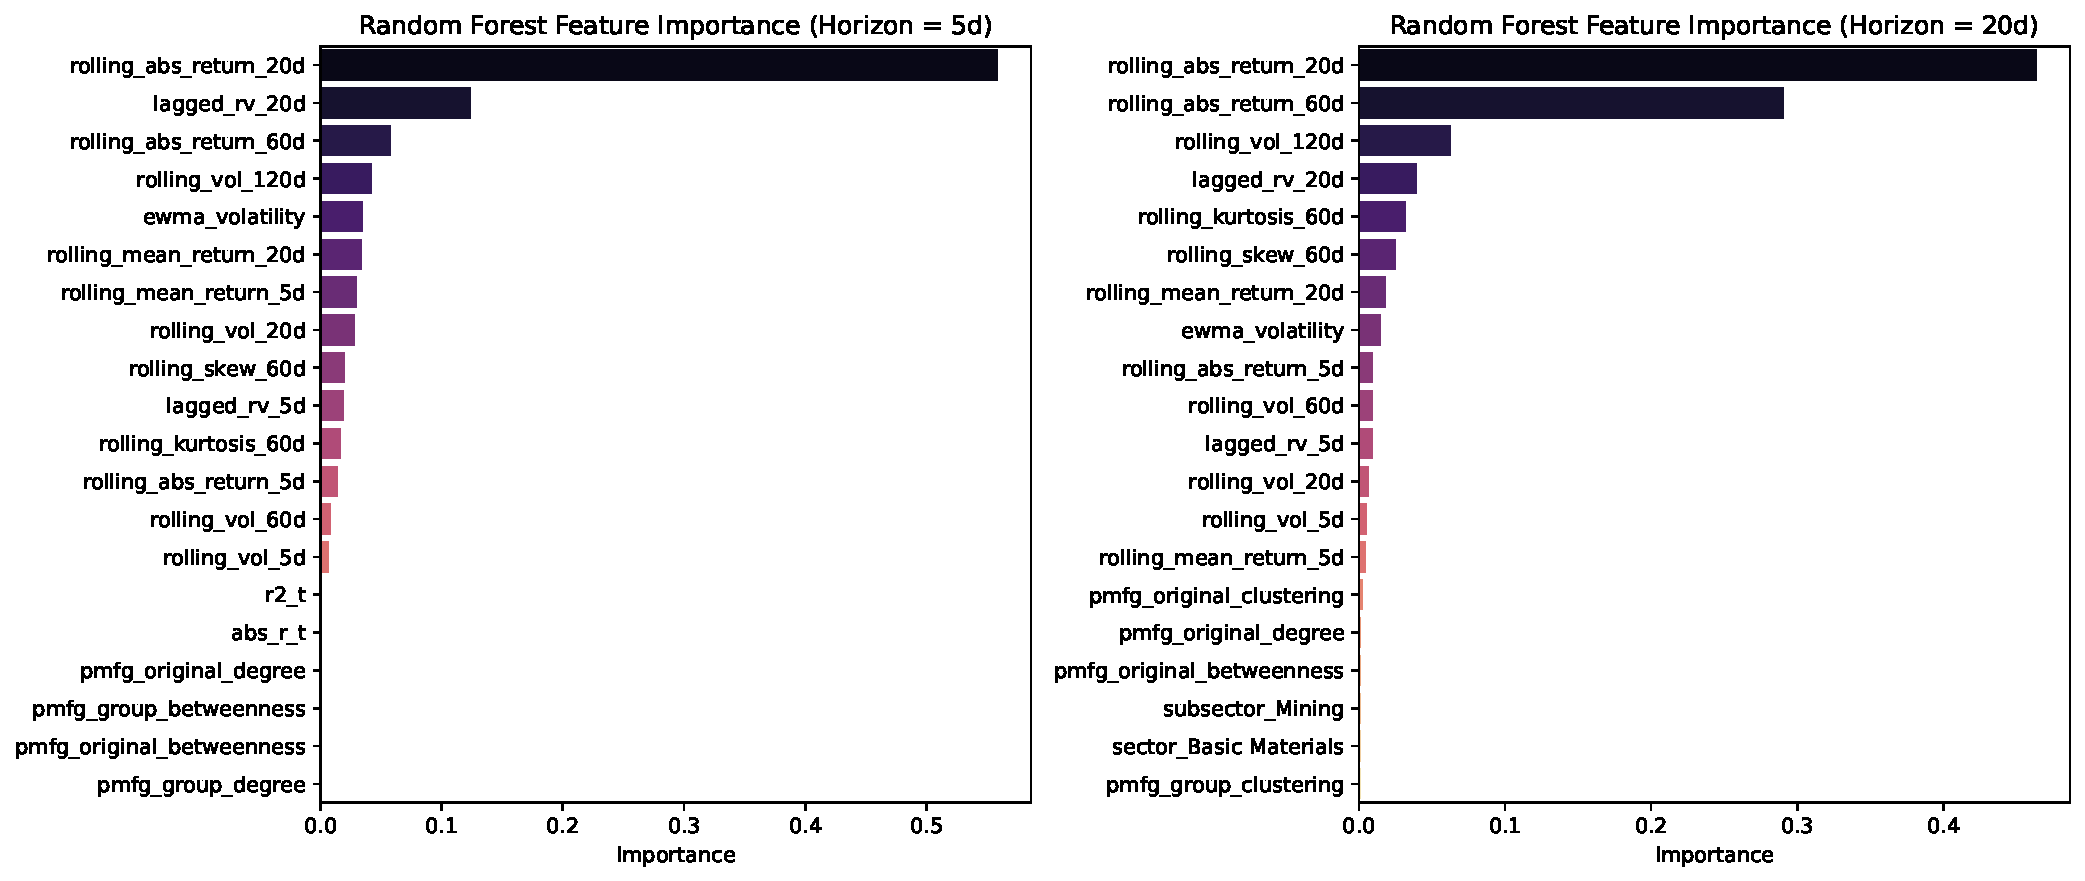
\includegraphics[
  width=0.95\linewidth,
  height=0.58\textheight,
  keepaspectratio
]{images/figure_18_ml_feature_importance.pdf}
\captionof{figure}{Feature importance for Random Forest volatility forecasting models. Classical volatility predictors dominate the selected rankings, while selected PMFG-based and sector/subsector variables appear with smaller but nonzero importance in the network-augmented feature set.}
\label{fig:feature_importance}
\end{center}

The strongest features are rolling absolute return over 20 days, lagged realized volatility and longer rolling volatility measures. Network features have smaller importance values than classical volatility predictors, but selected PMFG variables enter the top-ranked predictors, especially at the 20-day horizon. Because Random Forest importance measures can be affected by correlation among predictors, these rankings should be interpreted as model diagnostics rather than causal measures of variable relevance. The appropriate conclusion is therefore incremental: topology does not replace classical volatility features, but it may add structural information when included in a broader feature set.